\chapter{Sistemas de coordenadas: cilíndricas y esféricas}
\chaptermark{Coordenadas cilíndricas y esféricas}

\vspace{1cm}
\section{Sistemas de coordenadas}

\begin{tikzpicture}
	\fill [left color=red!50, right color=teal!50] (0,0) rectangle (3.5,.1);
	\fill [left color=teal!50, right color=blue!50] (3.5,0) rectangle (7.5,.1);
	\end{tikzpicture}
\vspace{0.5cm}


Para determinar una posición cualquiera $P$ del espacio necesitamos un \emph{\textbf{sistema de referencia}}, que consiste en un punto de referencia llamado \emph{origen}, $\mathcal O$ y unas direcciones de referencia respecto a los cuales representaremos la posición de $P$.

\begin{multicols}{2}
Desde $\mathcal O$ hasta $P$ trazamos el vector $\overrightarrow \mathcal OP$ que, como todo vector, tiene tres propiedades:
magnitud ($(d(\mathcal O,P)$), dirección (recta que pasa por $\mathcal O$ y $P$) y sentido (de $\mathcal O$ hacia $P$). Conocer $\overrightarrow{ \mathcal OP}$ es conocer estas tres propiedades, y viceversa.
\begin{figure}[H]
	\centering
	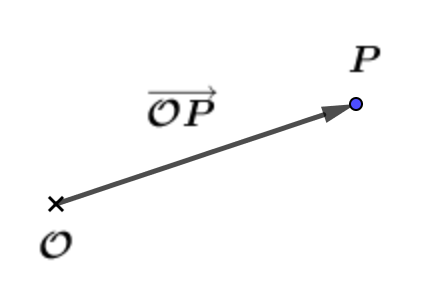
\includegraphics[width=.25\textwidth]{img-coordenadas/coordenadas-01.png}
\end{figure}	
\end{multicols}

Un \emph{\textbf{sistema de coordenadas}} es un método matemático para describir un vector libre. Dado $P$ y un sistema de referencia, existen distintos sistemas de coordenadas. A veces se usan distancias a los ejes coordenados, a veces se usan ángulos, a veces combinaciones de estos. Para cualquier $P$ y sistema de referencia, existen una variedad de sistemas de coordenadas alternativos.

Elegido el sistema de coordenadas, a cada punto del espacio se le asocia una terna de números, son sus \emph{coordenadas} en el sistema considerado. Y viceversa, a cualquier terna de números le corresponde un único punto del espacio.

El origen del sistema de referencia será el origen en nuestro sistema de coordenadas y en él todas las coordenadas tendrán valor nulo.

Sobre los ejes coordenados se definen unos \emph{vectores unitarios} (adimensionales), los \emph{versores}, que indican la dirección del eje que nos permetirán medir.


Los sistemas de coordenadas usuales son, en 2-D, las coordenadas cartesianas y las coordenadas polares (vistas en el tema anterior); en 3-D, las coordenadas cartesianas o rectangulares, las coordenadas cilíndricas y las coordenadas esféricas.

\vspace{1cm}
\color{teal}
\rule{250pt}{0.2pt}	

!`Ojo! Sistema de referencia $\neq$ sistema de coordenadas:\footnote{\textcolor{NavyBlue}{https://eltamiz.com/2011/05/04/mecanica-clasica-i-sistemas-de-referencia/}}

A veces, incluso en algunos libros de texto, se identifican los conceptos de sistema de referencia y sistema de coordenadas, pero ambos conceptos significan cosas distintas. Un sistema de referencia es un marco de observación, de modo que podamos tener en cuenta que lo que medimos depende de la posición y estado de movimiento de quien lo mide; por ejemplo, la descripción del movimiento de un satélite que orbita alrededor de la Tierra no es igual si la realizamos desde un punto de la superficie terrestre que desde la superficie de la Luna o el centro del Sol.

Por el contrario, un sistema de coordenadas no es más que la elección arbitraria de un conjunto de variables matemáticas que describen el movimiento. Un mismo sistema de referencia puede describir un movimiento utilizando varios conjuntos de coordenadas diferentes. Por ejemplo, el vuelo de una mosca en una habitación (observado desde la habitación considerada en reposo) puede describirse con coordenadas cartesianas $(x,y,z)$, con coordenadas esféricas $(r,\theta,\varphi)$ o con cualquier otro tipo de coordenadas que nos venga en gana, siempre que identifiquen de manera única cada posición de la mosca en la habitación.

Es decir, un sistema de referencia nos ayudará a determinar nociones de espacio como adelante, atrás, arriba, abajo en relación al punto de referencia que elijamos pero no nos dará valores cuantificados, ello sólo lo logremos usando un sistema de coordenadas que nos permita tomar medidas.
%\vspace{-15mm}
\begin{flushright}
\rule{250pt}{0.2pt}		
\end{flushright}

\color{black}


%\vspace{1cm}
\section{Cartesianas y Polares (2-D)}

\begin{tikzpicture}
	\fill [left color=red!50, right color=teal!50] (0,0) rectangle (3.5,.1);
	\fill [left color=teal!50, right color=blue!50] (3.5,0) rectangle (7.5,.1);
	\end{tikzpicture}
\vspace{0.5cm}

\begin{table}[H]
\centering
\begin{tabular}{ccc}
Coordenadas cartesianas & $\qquad$ & Coordenadas polares \\
$\boldsymbol{ \vec r=x\widehat i+y\widehat x}$ &  & $\boldsymbol{ \vec r=r\widehat r} \ \ (*)$ \\
$\widehat i,\ \widehat j$ constantes en todos los puntos &  & $\widehat r,\ \widehat \theta$ cambian (dirección) en cada punto \\
 & & $\widehat r=\widehat r (\theta);\ \ \widehat \theta= \widehat \theta(\theta)$ \\
c. cartesianas son \emph{homogéneas} &  & c. polares son \emph{no-homogéneas} 
\end{tabular}
\end{table}

$(*)$ Podríamos pensar que, en polares, la coordenada $r$ es suficiente para definir un vector y que la coordenada $\theta$ no afecta pero esto es falso ya que $\widehat r=\widehat(\theta)$

\begin{figure}[H]
	\centering
	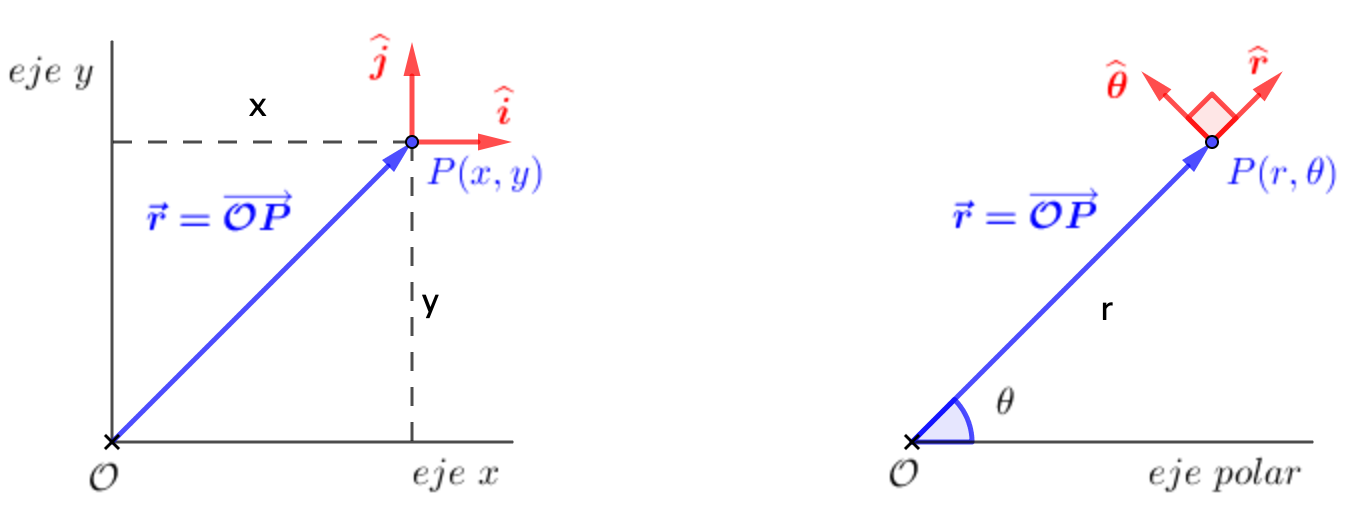
\includegraphics[width=.8\textwidth]{img-coordenadas/coordenadas-02.png}
\end{figure}	


\begin{table}[H]
\centering
\begin{tabular}{|ll|}
\hline
\multicolumn{2}{|c|}{\textbf{$\qquad$ Relación entre coordenadas cartesianas y polares. }}                          \\ \hline
\multicolumn{1}{|c|}{$\quad$ cartesianas $\to$ polares $\qquad$} & $\quad$ polares $\to$ cartesianas $\ \ $ \\ \hline
\multicolumn{1}{|c|}{} & \\
\multicolumn{1}{|c|}{$x=r\cos \theta$} & $\qquad \ \ r=\sqrt{x^2+y^2}$ \\ 
\multicolumn{1}{|c|}{} & \\
\multicolumn{1}{|c|}{$y=r\sin \theta$} & $\qquad \ \  \theta = \arctan \dfrac y x$ \\ 
\multicolumn{1}{|c|}{} & \\ \hline
\end{tabular}
\end{table}

\begin{multicols}{2}
	\begin{figure}[H]
	\centering
	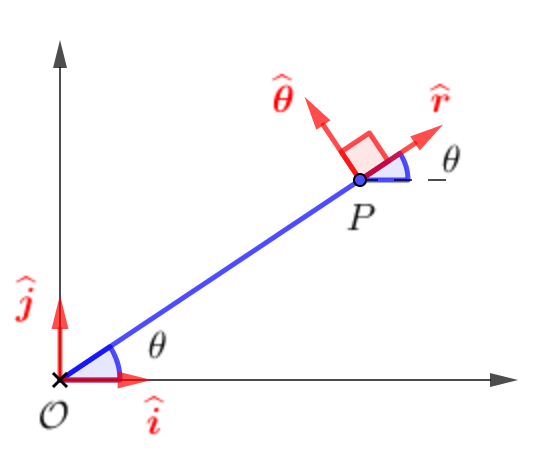
\includegraphics[width=.3\textwidth]{img-coordenadas/coordenadas-03.png}
	\end{figure}
	$\quad$
	
	De la figura:
	
	$\quad \widehat r=\vec u_r=\cos \theta \, \widehat i + \sin \theta \, \widehat j$
	
	$\quad \widehat \theta=\vec u_\theta=-\sin \theta \, \widehat i + \cos \theta \, \widehat j$
\end{multicols}

\color{gris}
Obviamente, $\ |\widehat i|=|\widehat j|=|\widehat r|=|\widehat \theta|=1;\ \ \widehat i \, \bot \, \widehat j;\ \ \widehat r \, \bot \, \widehat \theta$

Para el cambio inverso, dados los versores en polares encontrarlos en cartesianas podemos usar el álgebra. Las ecuaciones anteriores se pueden escribir matricialmente como 

$\qquad \mqty(\widehat r\\ \widehat \theta)= \mqty( \cos \theta & \sin \theta \\ -\sin \theta & \cos \theta) \mqty(\widehat i \\ \widehat j)=M\, \mqty(\widehat i \\ \widehat j)\, , \ $ premultiplicando por $M^{-1}\, , $

$\qquad \mqty(\widehat i \\ \widehat j)=M^{-1}\mqty(\widehat r \\ \widehat \theta)= \mqty( \cos \theta & -\sin \theta \\ \sin \theta & \cos \theta)
\mqty(\widehat r \\ \widehat \theta) \ \to \ \begin{cases}
 \ \widehat i= \cos \theta \, \widehat r-\sin \theta \, \widehat \theta \\	
  \ \widehat j= \sin \theta \, \widehat r+\cos \theta \, \widehat \theta
 \end{cases}$
\color{black}

\vspace{1cm}
\section{Coordenadas cartesianas en 3-D}

\begin{tikzpicture}
	\fill [left color=red!50, right color=teal!50] (0,0) rectangle (3.5,.1);
	\fill [left color=teal!50, right color=blue!50] (3.5,0) rectangle (7.5,.1);
	\end{tikzpicture}
\vspace{0.5cm}

\begin{multicols}{2}
\normalsize{$P(x,y,z)$, las} coordenadas son, respectivamente, las distancias de $P$ a los planos coordenados $YZ$, $XZ$ y $XY$. 

Los vectores unitarios (versores) son ahora $\widehat i, \, \widehat j,\, \widehat k$

Por convenio (física) los versores se toman de modo que se cumple que:

$\qquad  \widehat i \times \widehat j=\widehat k;\ \ \widehat j \times \widehat k=\widehat i;\ \ \widehat k \times \widehat i=\widehat j$
\begin{figure}[H]
	\centering
	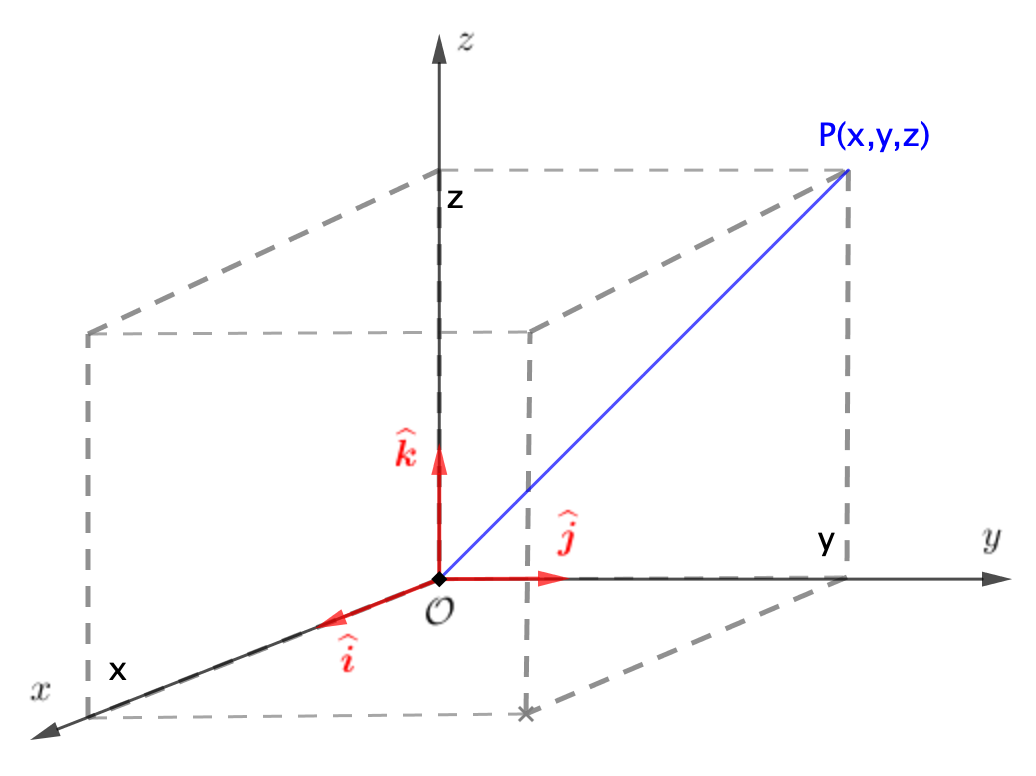
\includegraphics[width=.5\textwidth]{img-coordenadas/coordenadas-04.png}
	\end{figure}	
\end{multicols}

\vspace{7mm}
\subsection{Variación infinitesimal de las coordenadas}
\vspace{-5mm}
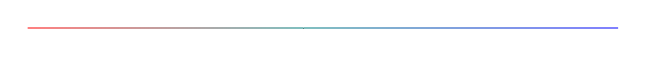
\begin{tikzpicture}
	\fill [left color=red!50, right color=teal!50] (0,0) rectangle (3.5,.01);
	\fill [left color=teal!50, right color=blue!50] (3.5,0) rectangle (7.5,.01);
	\end{tikzpicture}
\vspace{0.5cm}

\begin{multicols}{2}
\normalsize{Si} las coordenadas de un punto $P(x,y,z)$ varían infinitesimalmente, la variación en el vector de posición será:

$\qquad \dd \vec r=\dd x\, \widehat i +\dd y\, \widehat j +\dd z\, \widehat k$

\begin{small}El punto habrá recorrido un diferencial de arco\end{small}\normalsize{:}

$\qquad \dd  s = \sqrt{(\dd x)^2+(\dd y)^2+(\dd z)^2}$
	\begin{figure}[H]
	\centering
	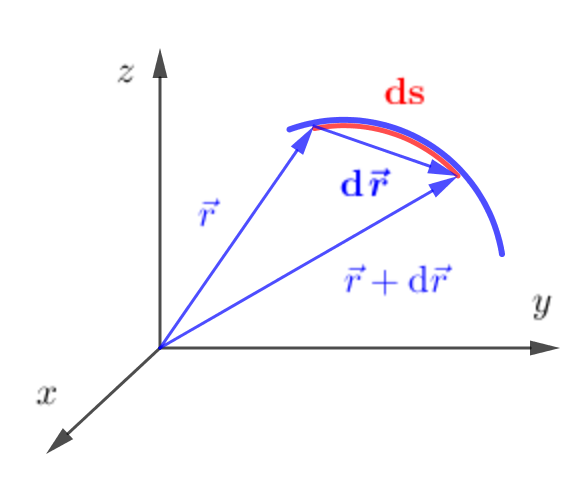
\includegraphics[width=.35\textwidth]{img-coordenadas/coordenadas-05.png}
	\end{figure}
\end{multicols}

\vspace{0.5cm}
\begin{multicols}{2}
$\quad$

\normalsize{Elemento} diferencial de superficie:

$\qquad \overrightarrow{\dd A}=\dd A_x \, \widehat i+\dd A_y \, \widehat j+\dd A_z \, \widehat k$

Proyectando sobre los planos coordenados:

$\qquad \overrightarrow{\dd A}=\dd y \, \dd z \, \widehat i+\dd x \, \dd z \, \widehat j+ \dd x \, \dd y \, \widehat k$
	\begin{figure}[H]
	\centering
	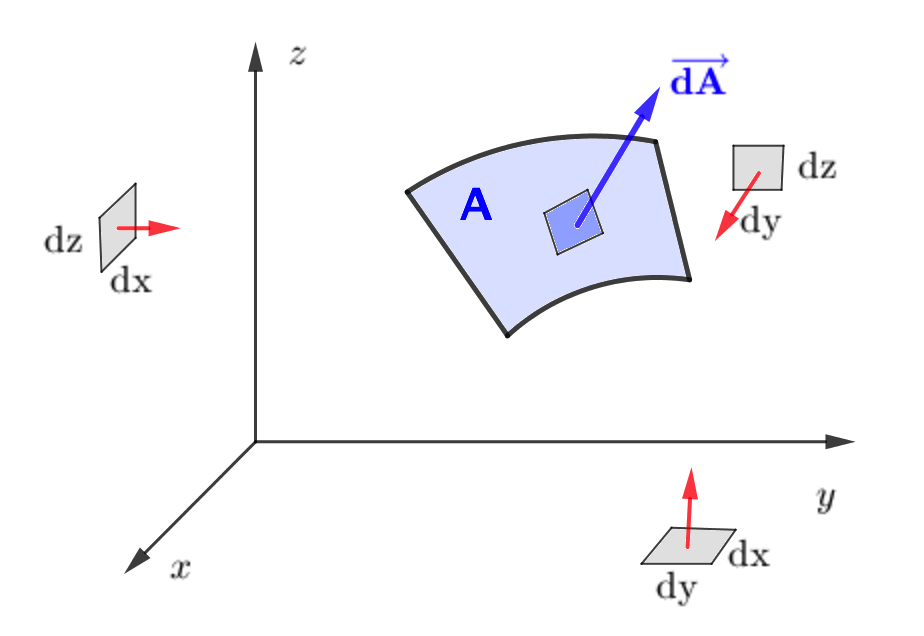
\includegraphics[width=.4\textwidth]{img-coordenadas/coordenadas-06.png}
	\end{figure}
\end{multicols}

\vspace{0.5cm}
\begin{multicols}{2}
$\quad$

\normalsize{E}lemento diferencial de volumen: es un paralelepípedo de aristas $\dd x,\ \dd y \text{ y } \dd z$

$\qquad \dd V=\dd x \, \dd y\, \dd z$
	\begin{figure}[H]
	\centering
	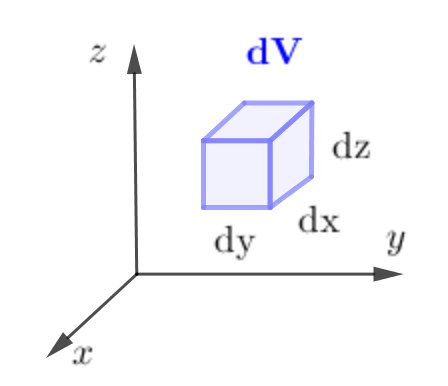
\includegraphics[width=.3\textwidth]{img-coordenadas/coordenadas-07.png}
	\end{figure}
\end{multicols}


\vspace{1cm}
\section{Coordenadas cilíndricas}

\begin{tikzpicture}
	\fill [left color=red!50, right color=teal!50] (0,0) rectangle (3.5,.1);
	\fill [left color=teal!50, right color=blue!50] (3.5,0) rectangle (7.5,.1);
	\end{tikzpicture}

\vspace{0.5cm}

\begin{multicols}{2}
\normalsize{Es} un sistema de coordenadas alternativo para describir puntos en 3D. Se usa como referencia un plano que pasa por el punto $\mathcal O$ O. 

La proyección del punto $P$ sobre este plano se describe con coordenadas `polares' $\rho \text{ y } \theta$. La tercera coordenada, usualmente llamada $z$, es simplemente la distancia entre $P$ y el plano de referencia. 

	\begin{figure}[H]
	\centering
	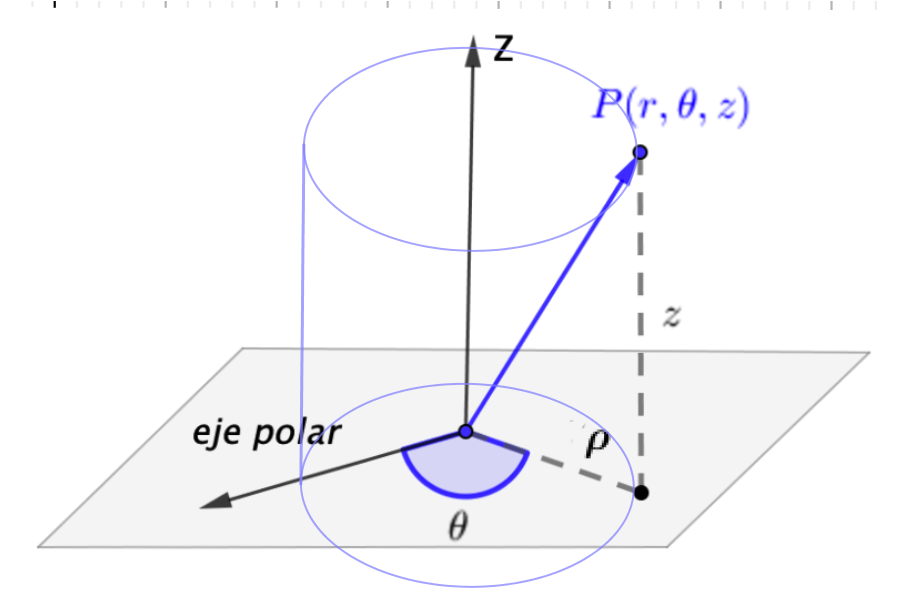
\includegraphics[width=.4\textwidth]{img-coordenadas/coordenadas-08.png}
	\end{figure}
\end{multicols}
Los vectores unitarios, versores, en este sistema son la tríada $(\widehat \rho,\, \widehat \theta,\, \widehat k)$.

El coordenadas cilíndricas el vector de posición $\vec r$  se expresa como: $\quad \vec r=\rho\, \widehat \rho+z\, \widehat k$.

El sistema de coordenadas cilíndricas en no-homogéneo, los versores no son constantes, en este caso, $\widehat \rho=\widehat \rho(\theta)$.


\begin{multicols}{2}


$x= \rho \cos \theta;\quad y=\rho \sin \theta;\quad z=z$

$\vec r=\rho \cos \theta \, \widehat i+\rho \sin \theta \, \widehat j+z \, \widehat k=\rho \, \widehat \rho+z \, \widehat k$

$\widehat \rho= \vec u_\rho=\rho \cos \theta \, \widehat i+\rho \sin \theta \, \widehat j$

$\widehat \theta=-\sin \theta \, \widehat i+\cos \theta \, \widehat j$

$\widehat k=\widehat k$

\begin{figure}[H]
	\centering
	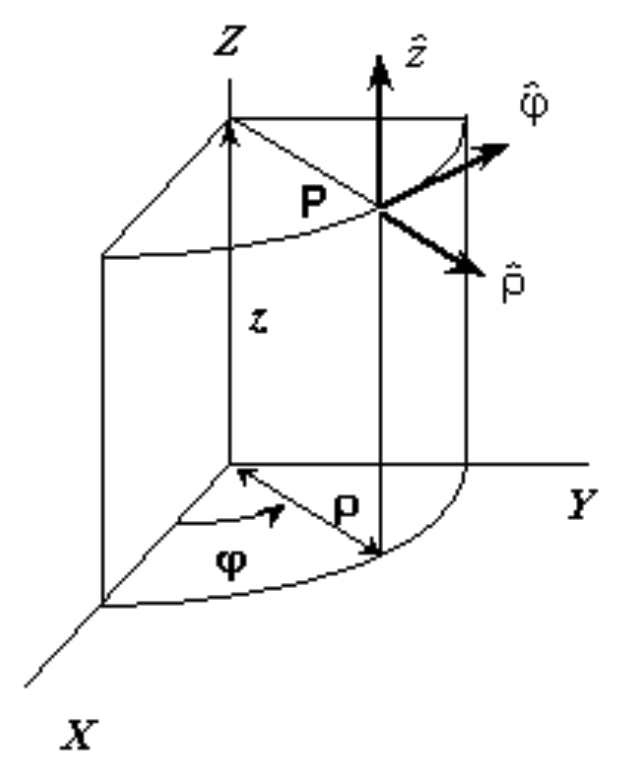
\includegraphics[width=.25\textwidth]{img-coordenadas/coordenadas-11.png}
	\end{figure}
	
\end{multicols}

\vspace{1cm}
\section{Coordenadas esféricas}

\begin{tikzpicture}
	\fill [left color=red!50, right color=teal!50] (0,0) rectangle (3.5,.1);
	\fill [left color=teal!50, right color=blue!50] (3.5,0) rectangle (7.5,.1);
	\end{tikzpicture}

\vspace{0.5cm}


En coordenadas esféricas, la primera coordenada es la distancia entre $P$ y el origen $\mathcal O$, que llamaremos $r$. Las dos coordenadas adicionales son  ángulos: como en coordenadas cilíndricas se define también un plano de  referencia que pasa por el punto $\mathcal O$ y , contenido en él, un eje llamado \emph{eje azimutal}. El ángulo entre este eje y la proyección de $P$ sobre el plano define la coordenada llamada \emph{ángulo azimutal}, $\varphi$. Perpendicular al plano mencionado y pasando por $\mathcal O$ se define un segundo eje de referencia, el \emph{eje cenital}. El ángulo entre este eje y el vector posición es la tercera coordenada,el \emph{ángulo cenital}, $\theta$. 

\begin{multicols}{2}
$\quad$

La terna orientada de vectores unitarios en este caso es $(\widehat r,\, \widehat \varphi,\, \widehat \theta)$.

El esféricas, el vector de posición $\vec r$  se expresa como: $\quad \vec r=r\, \widehat r$.

El sistema de coordenadas cilíndricas en no-homogéneo, los versores no son constantes, en este caso, $\widehat r=\widehat r(\varphi, \theta), \,  \varphi=\widehat r(\varphi, \theta),\,  \theta=\widehat r(\varphi, \theta)$.

\begin{figure}[H]
	\centering
	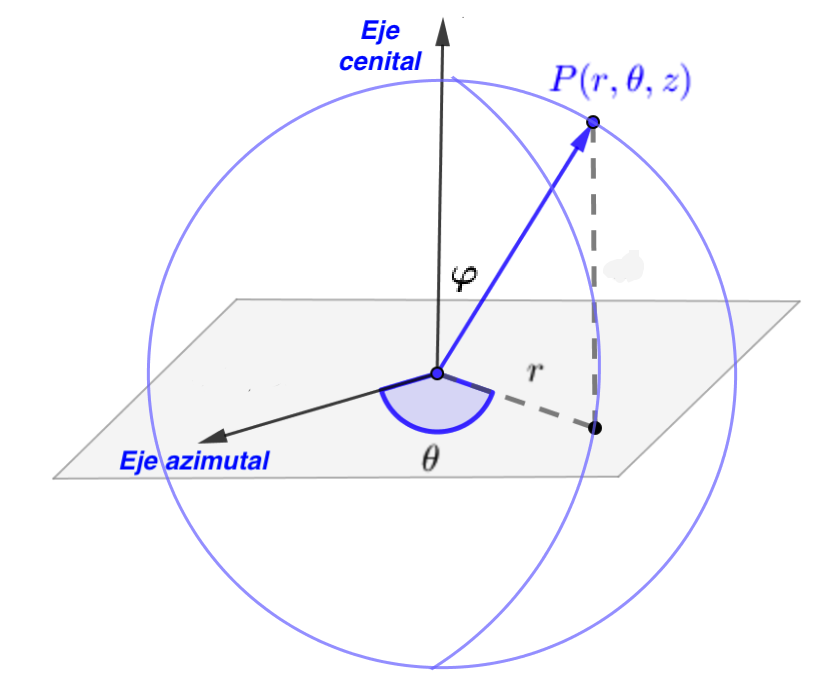
\includegraphics[width=.45\textwidth]{img-coordenadas/coordenadas-09.png}
	\end{figure}
	
\end{multicols}



\begin{multicols}{2}
$\quad$

$x=r\sin \theta \cos \varphi;\ y=r\sin \theta \sin \varphi,\ z=r\cos \theta$

$\vec r= r\sin \theta \cos \varphi\, \widehat i+ r\sin \theta \sin \varphi\, \widehat j+ r\cos \theta \, \widehat k = r\, \widehat r$

\vspace{3mm}
$\widehat r= \cos \varphi \sin \theta \, \widehat i+ \sin \varphi \sin \theta º, \widehat j+ \cos \theta \, \widehat k$

$\widehat \theta= \cos \varphi \cos \theta \, \widehat i+ \sin \varphi \cos \theta \, \widehat j- \sin \theta \, \widehat k$

$\widehat \varphi= -\sin \varphi\, \widehat i + \cos \varphi \, \widehat j$

\begin{figure}[H]
	\centering
	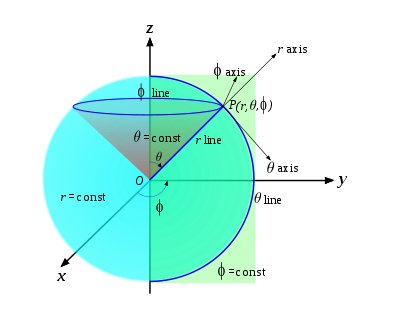
\includegraphics[width=.5\textwidth]{img-coordenadas/coordenadas-10.png}
	\end{figure}

\end{multicols}

\underline{Observación}: En esféricas se usa la coordenada $r$ que mide la distancia entre $P$ y $\mathcal O$, en cambio, en cilíndricas la coordenada $\rho$ mide la distancia de $P$ al plano de referencia.



\vspace{1cm}
\section{Variación infinitesimal de las coordenadas cilíndricas y esféricas}

\begin{tikzpicture}
	\fill [left color=red!50, right color=teal!50] (0,0) rectangle (3.5,.1);
	\fill [left color=teal!50, right color=blue!50] (3.5,0) rectangle (7.5,.1);
	\end{tikzpicture}
\vspace{0.5cm}

\begin{figure}[H]
	\centering
	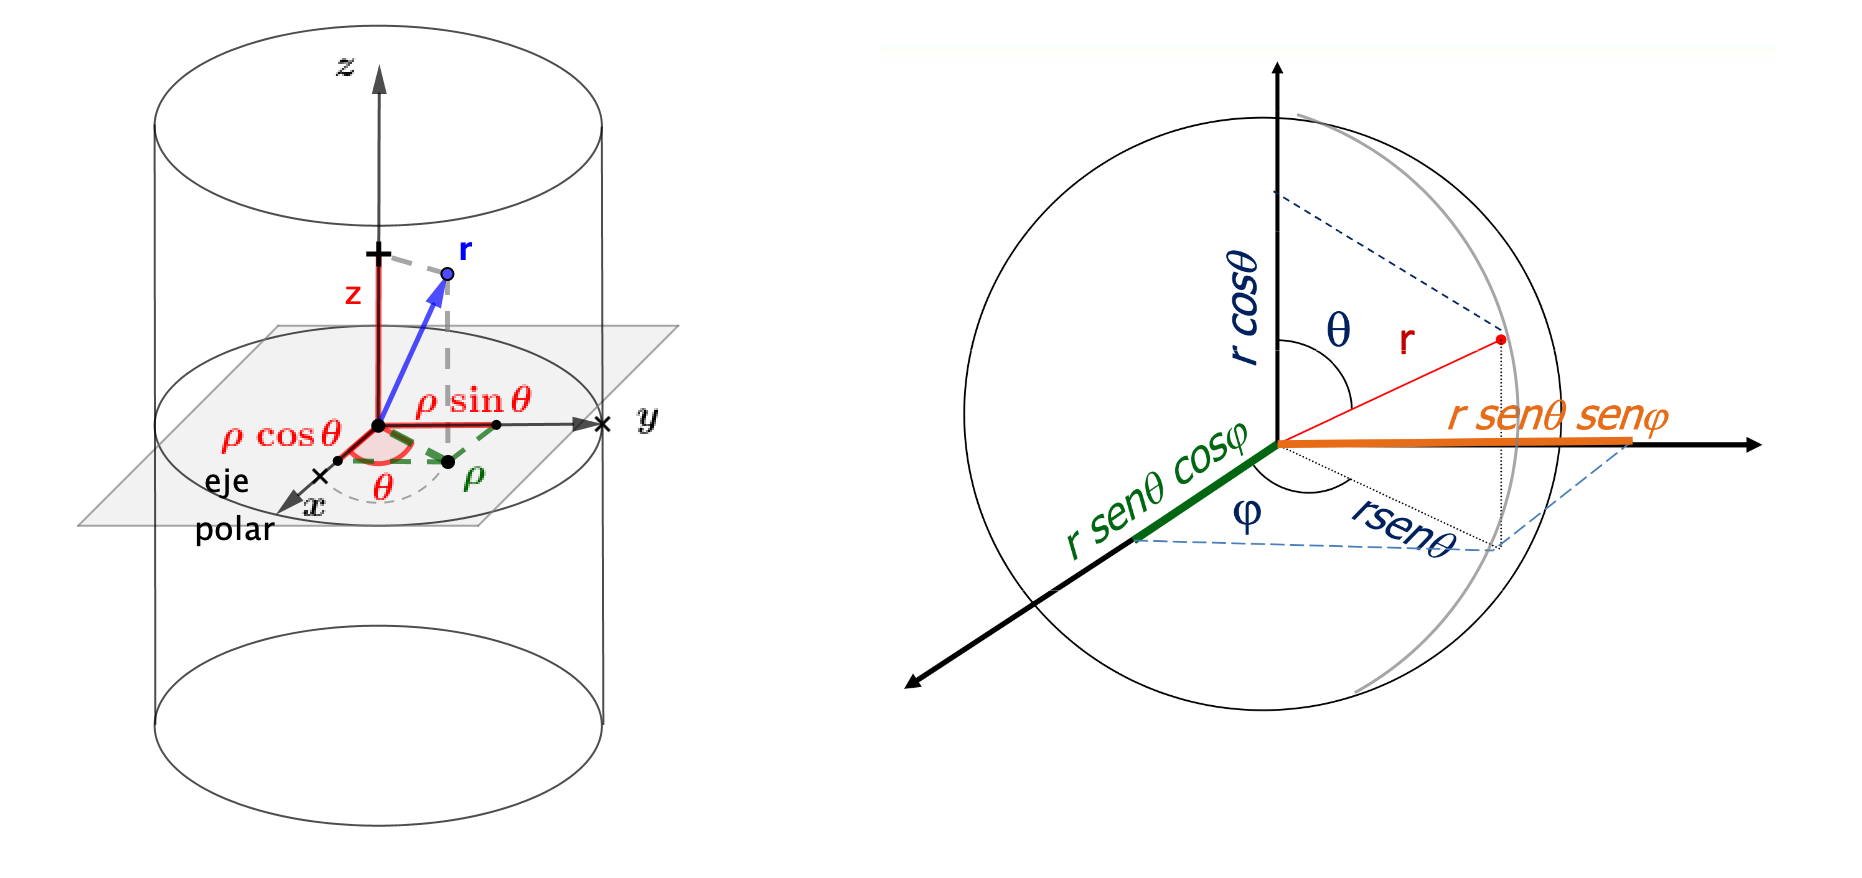
\includegraphics[width=.95\textwidth]{img-coordenadas/coordenadas-14.png}
	\end{figure}

\begin{table}[H]
\centering
\begin{tabular}{|c|c|}
\hline
\textbf{$\qquad$ C.  cilíndricas $\qquad$ } & \textbf{$\qquad$  C. esféricas $\qquad$ } \\ \hline
	$\overrightarrow{\mathrm{dA}}=\rho \mathrm{d} \theta \, \mathrm{d} z\, \widehat r$  
&     $\overrightarrow{\mathrm{dA}}=r \sin \theta \mathrm{d} \varphi\, r \mathrm{d} \theta \, \mathrm{d} r$    \\ \hline
	$\mathrm{d}V=\rho \mathrm{d}\theta\, \mathrm{d} z\, \mathrm{d} r$        
&     $\mathrm{d}V=r\sin \theta \mathrm{d}\varphi\, r\mathrm{d}\theta\, \mathrm{d}r$   \\ \hline
\end{tabular}
\end{table}

\begin{multicols}{2}
\begin{figure}[H]
	\centering
	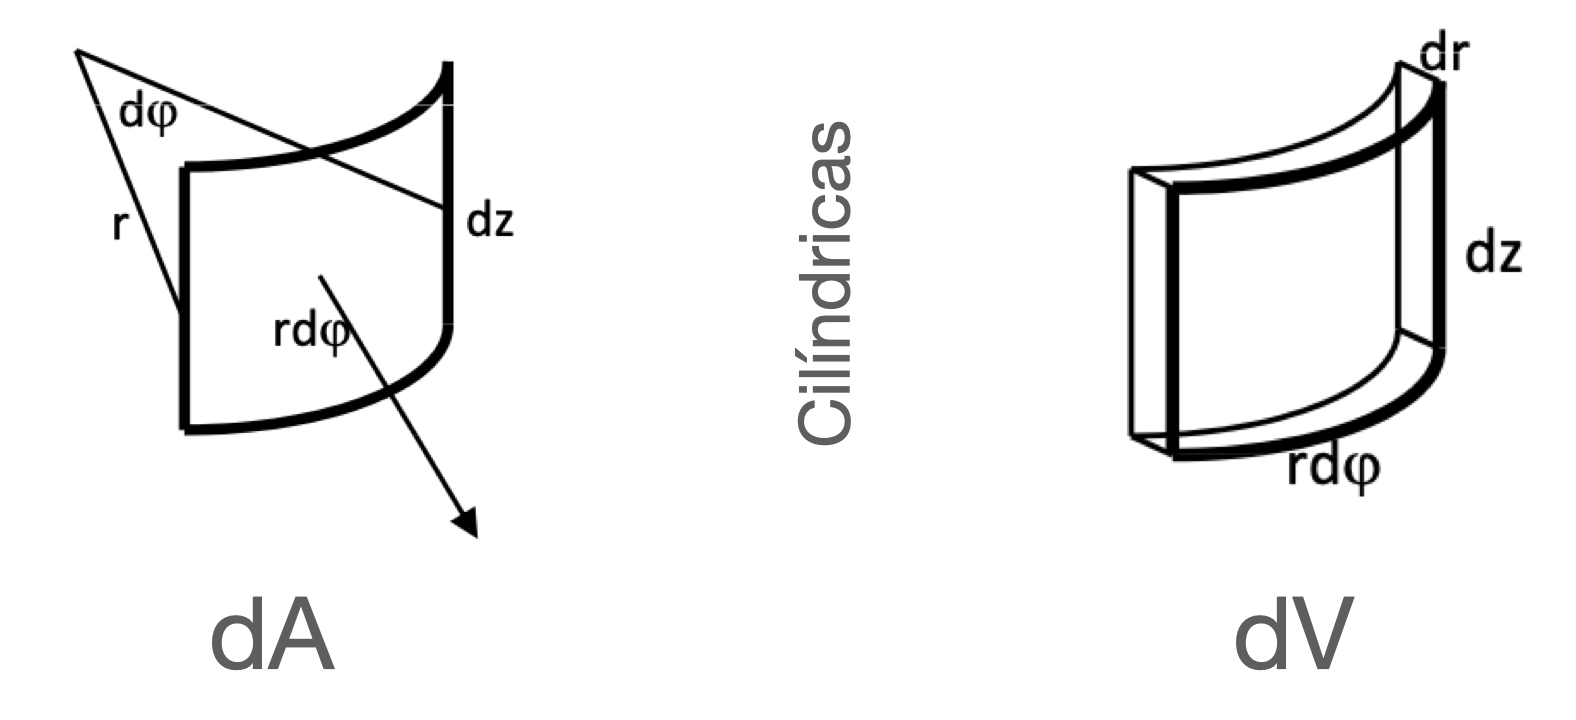
\includegraphics[width=.5\textwidth]{img-coordenadas/coordenadas-12.png}
	\end{figure}
	
\begin{figure}[H]
	\centering
	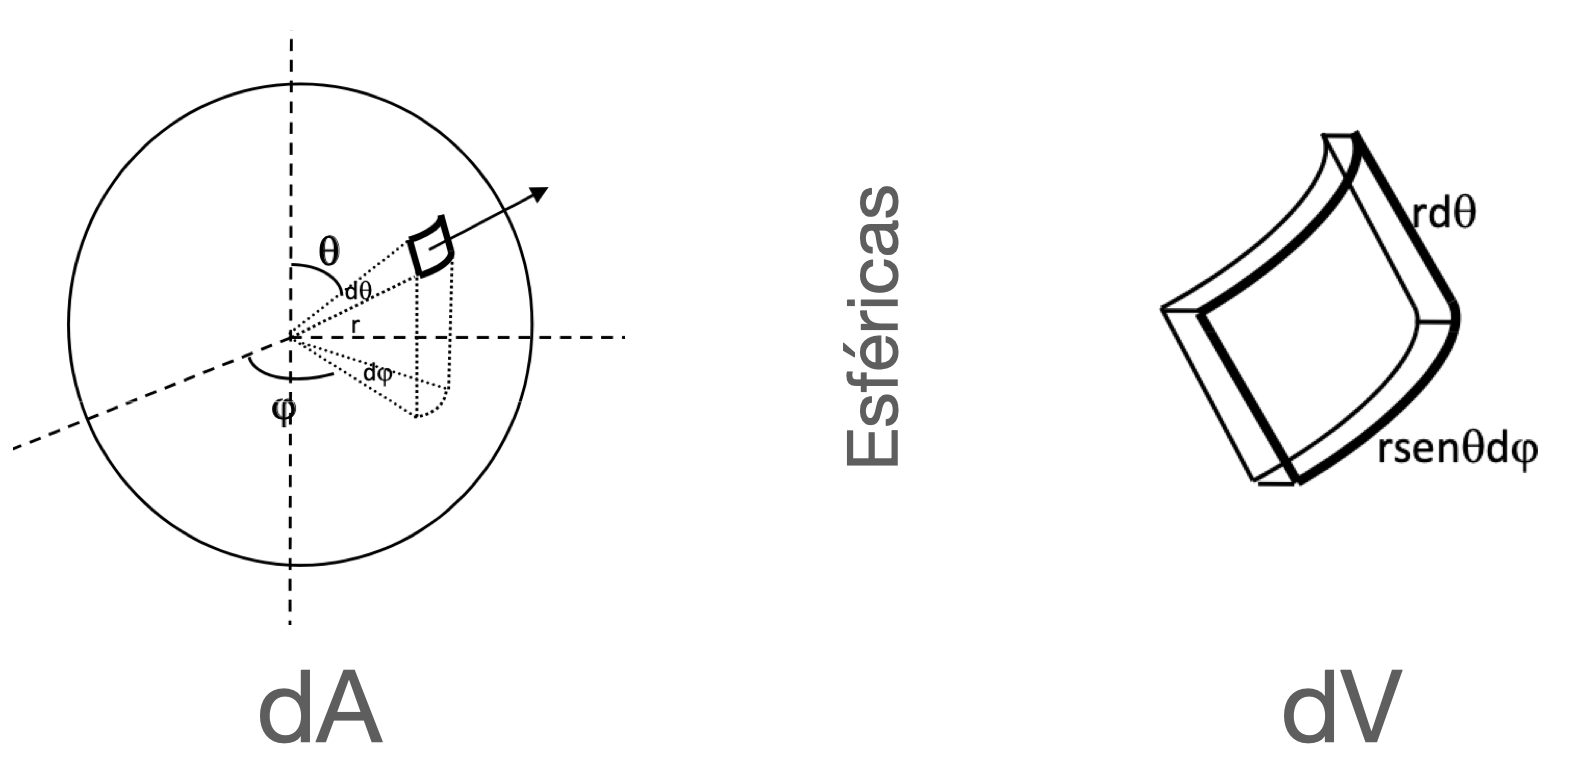
\includegraphics[width=.45\textwidth]{img-coordenadas/coordenadas-13.png}
	\end{figure}
\end{multicols}

\begin{comment}

%%%%%%%%%%%%%%%%%%%%%%%%%%%%%%%%%%%. SECCIONES
\chapter{texto}

\begin{tikzpicture}
	\fill [left color=red!50, right color=teal!50] (0,0) rectangle (6.5,.2);
	\fill [left color=teal!50, right color=blue!50] (6.5,0) rectangle (11.5,.2);
	\end{tikzpicture}

\vspace{1cm}
\section{texto}

\begin{tikzpicture}
	\fill [left color=red!50, right color=teal!50] (0,0) rectangle (3.5,.1);
	\fill [left color=teal!50, right color=blue!50] (3.5,0) rectangle (7.5,.1);
	\end{tikzpicture}
\vspace{0.5cm}

\vspace{5mm}
\subsection{texto}
\vspace{-5mm}
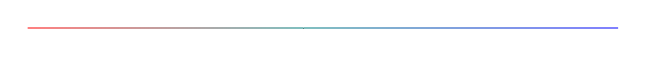
\begin{tikzpicture}
	\fill [left color=red!50, right color=teal!50] (0,0) rectangle (3.5,.01);
	\fill [left color=teal!50, right color=blue!50] (3.5,0) rectangle (7.5,.01);
	\end{tikzpicture}
\vspace{0.5cm}


%%%%%%%%%%%%%%%%%%%%%%%%%%%%%%%%%%%. \begin{ ------>. 
detsacado;  cuadro-naranja;  cuadro-gris;  miejercicio (solución extensa);  mipropuesto (solución corta y fuera del cuadro)

%%%%%%%%%%%%%%%%%%%%%%%%%%%%%%%%%%%. CURIOSIDAD
\vspace{1cm}
\color{ForestGreen!80}
\rule{250pt}{0.2pt}
Texto
\vspace{-8mm}
\begin{flushright}
\rule{250pt}{0.2pt}		
\end{flushright}	
\color{black}
\end{comment}
